
\documentclass[UTF8, onecolumn, a4paper]{article}
\usepackage{ctex}
\setlength{\parindent}{2em}
\usepackage{appendix}
\usepackage{geometry}
\usepackage{amsmath, amsthm}
\usepackage{multirow, multicol}
\usepackage{subfigure}
\usepackage{float}
\usepackage{graphicx}
\usepackage{lettrine}
\usepackage{authblk}
\usepackage{booktabs}
\usepackage{indentfirst}
\usepackage{xcolor, fontspec}%用于设置颜色
\usepackage[ruled,vlined]{algorithm2e}
\usepackage{listings}%用于显示代码
\usepackage[colorlinks,
linkcolor=red,
anchorcolor=blue,
citecolor=green
]{hyperref}
\usepackage{tikz}
\usepackage{dirtree}
\usetikzlibrary{trees}
\geometry{left=3.0cm,right=3.0cm,top=2.0cm,bottom=2.0cm}

%\title{\textbf{数字图像处理: Homework 1}}%———总标题
\title{	
	\normalfont\normalsize
	\textsc{Tsinghua University, Department of Computer Science and Technology}\\ % Your university, school and/or department name(s)
	\vspace{15pt} % Whitespace
	\rule{\linewidth}{2.0pt}\\ % Thick top horizontal rule
	\vspace{17pt} % Whitespace
	{\LARGE \textbf{Efficient Gradient-Domain Compositing Using Quadtrees}}\\ % The assignment title
	\vspace{4pt} % Whitespace
	\rule{\linewidth}{1.5pt}\\ % Thick bottom horizontal rule
	\vspace{2pt} % Whitespace
}

\author{刘泓尊\quad 2018011446\quad 计84}
%\affil{Department of Computer Science, Tsinghua University}

\begin{document}
\maketitle
\lstset{%代码块全局设置
	backgroundcolor=\color{red!3!green!3!blue!3},%代码块背景色为浅灰色
	rulesepcolor= \color{gray}, %代码块边框颜色
	breaklines=true,  %代码过长则换行
	numbers=left, %行号在左侧显示
	numberstyle= \small,%行号字体
	%keywordstyle= \color{red},%关键字颜色
	commentstyle=\color{gray}, %注释颜色
	frame=shadowbox,%用方框框住代码块
	xleftmargin=1em,
	xrightmargin=0em,
	tabsize=5,
	%rulesepcolor=\color{red!20!green!20!blue!20},  %阴影颜色
	keywordstyle={\color{blue!90!}\fontspec{Consolas Bold}},   %关键字颜色
	commentstyle={\color{blue!70!black}\fontspec{Consolas Italic}},   %注释颜色
	stringstyle=\color{orange!100!black}, %字符串颜色
	numberstyle=\color{purple}, %行号颜色
	%basicstyle=\ttfamily, %代码风格
	basicstyle=\fontspec{Consolas},
	showstringspaces=false,          % underline spaces within strings only  
	showtabs=false,
	captionpos=t, %文件标题位置
	flexiblecolumns
}

\section{算法介绍}
该算法\cite{quadtree}提供一种高效的图像融合手段,利用四叉树划分图像区间,使得四叉树的一个节点的解可以近似代替该区域所有像素的解,从而将算法时间复杂度从$O(n)$降低到$O(p)$, 其中$n$是融合区域的像素个数,$p$是融合边界的长度,使得算法复杂度接近线性。

该算法没有直接去解图像融合的泊松方程$Ax = b$, 而是考虑到最终解和被嵌入区域的差值$x_{\delta}$, 即$x = x_0 + x_{\delta}$. 
那么考虑到$Ax = b$的最小二乘解,可以转换为求解:
$$A^TAx_{\delta} = A^T(b - Ax_0)$$
因为图像有局部性连续的特征,可以认为$(b - Ax_0)$在离融合边界远的区域均接近0,所以可以利用四叉树缩点来降低求解方程的规模。

假设四叉树缩点之后图像有$y$个关键点,那么我们希望全部像素$x$能够是$y$的线性组合,即存在矩阵$S$使得$x = Sy$。关于$S$的构造,可以采用双线性插值的方法,四叉树节点所覆盖区域中的像素就是其区域四个顶点像素值的线性插值。从而上述方程可以转换为:
$$S^TA^TASy_{\delta} = S^TA^T(b - ASy_0)$$

在构建四叉树之后,等式右侧的$S^TA^T(b - ASy_0)$遍历一遍四叉树即可求得。而等式左边的 $S^TA^TAS$也可以在遍历过程中沿着四叉树节点的边缘对每对相邻像素之间的梯度加权求和。所以算法开销就是遍历四叉树与求解线性方程组的总和。

算法流程如下:
\begin{enumerate}
	\item 根据融合区域边界和图像边界构建四叉树
	\item 遍历四叉树得到关键点,并建立矩阵$S$和矩阵$AS$, 以及等式右边的$(b - ASy_0)$
	\item 利用最小二乘法求解$ASy_{\delta} = (b - ASy_0)$的最优解
	\item 根据$y_{\delta}$还原每个像素值,融合
\end{enumerate}

\section{实例}
我选择了春季学期“数字图像处理”课程提供的若干测例,每个测例包括被融合图、融合图以及mask图用于标注融合边界。

表\ref{table:table1}展示了这两个测例需要的时间和大致存储空间(用存储线性方程组所占用空间近似计算)的对比,以及优化后相对于优化前的精确解的均方误差RMS(average per-pixel root-mean-square error)以及R通道上的最大误差(max error on R channel)。

\begin{table}[h]
	\centering
	\caption{两个例子的性能对比与误差统计}
	\label{table:table1}
	\begin{tabular}{c|p{1.3cm}p{1.3cm}p{1.5cm}p{1.5cm}p{1.5cm}p{1.5cm}p{1.3cm}}
	\toprule
	& 优化前用时(s) & 优化后用时(s) & 优化前空间(MB) & 优化后空间(MB) & 均方误差 & 最大误差(R通道) & 融合区域像素 \\
	\midrule
	Example1 & 67.32 & \textbf{0.87} & 2.508 & \textbf{0.036} & 0.002 & 1.000 & 360*266 \\
	\hline
	Example2 & 15.49 & \textbf{0.50} & 1.135 & \textbf{0.034} & 0.094 & 1.000 & 120*180 \\
	\bottomrule
	\end{tabular}
\end{table}

\begin{figure}[H]
	\centering
	\subfigure[Source]{
		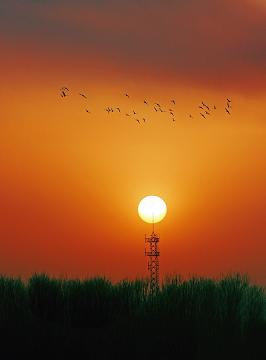
\includegraphics[width=0.2\linewidth]{../pic/test1_src}
	}
	\subfigure[Mask]{
		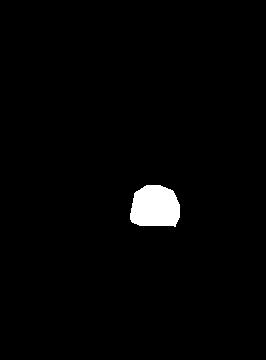
\includegraphics[width=0.2\linewidth]{../pic/test1_mask}
	}
	\subfigure[Target]{
		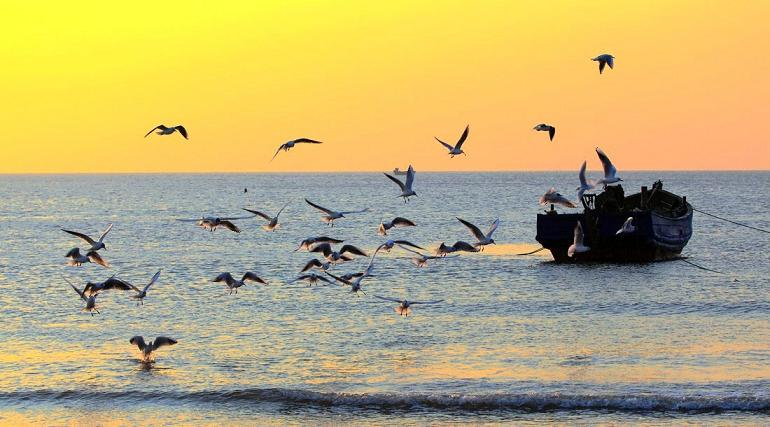
\includegraphics[width=0.4\linewidth]{../pic/test1_target}
	}
	
	\subfigure[Naive Copy]{
		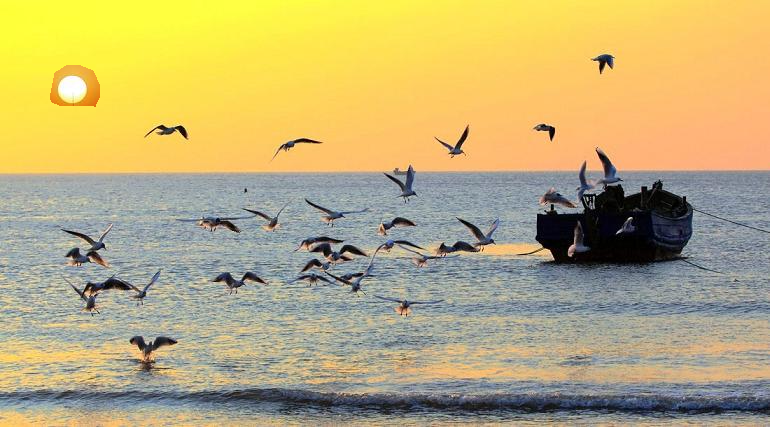
\includegraphics[width=0.4\linewidth]{../src/example1/copy}
	}
	\subfigure[Full Poisson]{
		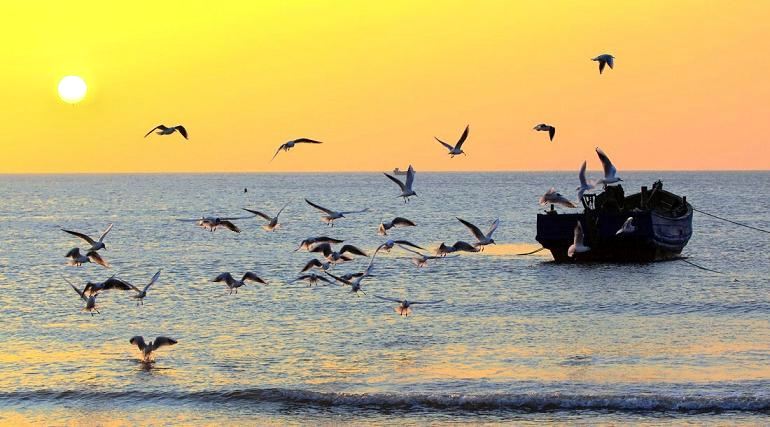
\includegraphics[width=0.4\linewidth]{../src/example1/full}
	}
	\subfigure[Quadtree Poisson]{
		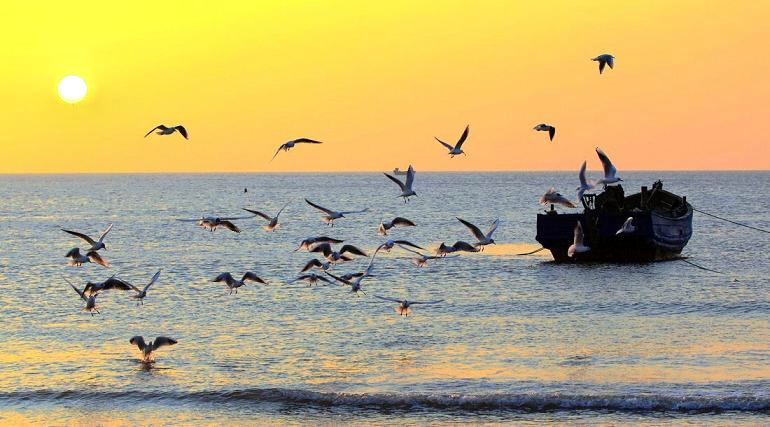
\includegraphics[width=0.4\linewidth]{../src/example1/quad}
	}
	\subfigure[Quadtree]{
		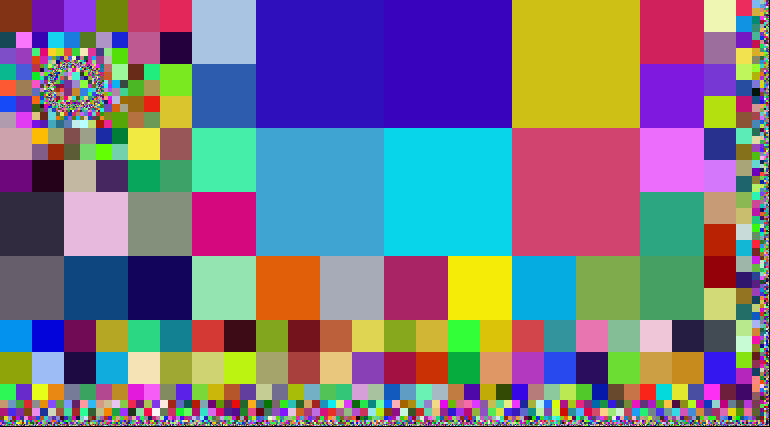
\includegraphics[width=0.4\linewidth]{../src/example1/tree}
	}
	\caption{Image Fusion Example 1 (“Full Poisson”即使用优化前的求解全像素泊松方程的结果;“Quadtree Poisson”是使用四叉树优化之后的算法结果;“tree”是构建的四叉树可视化示意图)}
	\label{fig:Fusion1}
\end{figure}

\begin{figure}[H]
	\centering
	\subfigure[Source]{
		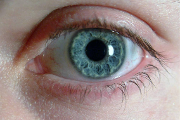
\includegraphics[width=0.3\linewidth]{../pic/test2_src}
	}
	\subfigure[Mask]{
		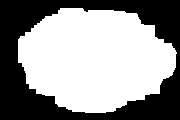
\includegraphics[width=0.3\linewidth]{../pic/test2_mask}
	}
	\subfigure[Target]{
		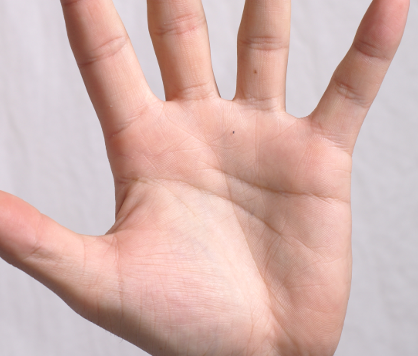
\includegraphics[width=0.3\linewidth]{../pic/test2_target}
	}
	
	\subfigure[Naive Copy]{
		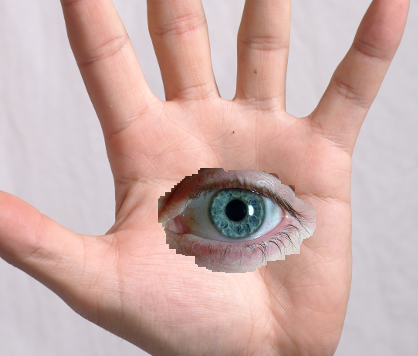
\includegraphics[width=0.4\linewidth]{../src/example2/copy}
	}
	\subfigure[Full Poisson]{
		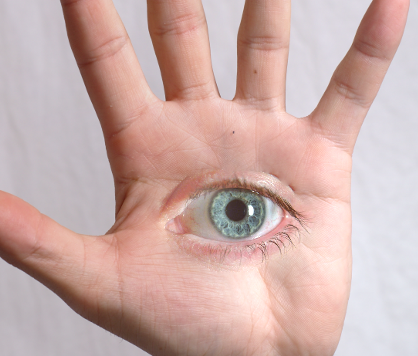
\includegraphics[width=0.4\linewidth]{../src/example2/full}
	}
	\subfigure[Quadtree Poisson]{
		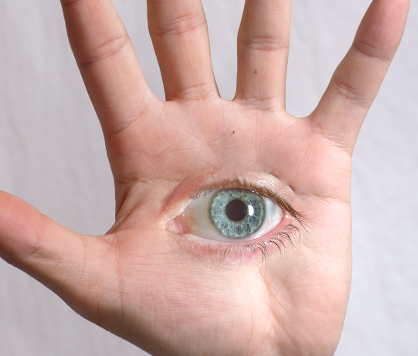
\includegraphics[width=0.4\linewidth]{../src/example2/quad}
	}
	\subfigure[Quadtree]{
		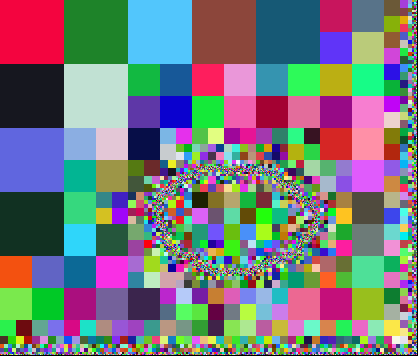
\includegraphics[width=0.4\linewidth]{../src/example2/tree}
	}
	\caption{Image Fusion Example 2}
	\label{fig:Fusion2}
\end{figure}

可以看到使用四叉树优化之后的融合结果与优化前的结果在肉眼上没有明显区别,融合区域平滑自然。对于构造的四叉树特征,可以看到在离融合边界较远的区域,四叉树节点较大;而融合边界和图像边界都使得四叉树节点逐渐缩小到一个像素范围,和前面的分析是一致的。

从表\ref{table:table1}可以看到,使用四叉树优化之后的算法复杂度大幅缩减,在两个测例上的时间和空间开销都有了100倍的提升。相当于精确解,使用四叉树优化的近似解误差很小,任一像素的误差都不超过1.0。

\bibliographystyle{plain}%规定参考文献的样式
\bibliography{reference}  %参考文献库的名字Ref

\appendix
\section{运行说明}
\texttt{src/}文件夹下是本项目源码,同时提供了\texttt{Makefile}方便编译。
\begin{enumerate}
	\item 本项目使用了\texttt{eigen3}库用以加速方程求解,运行前需要自行配置
	\item 测试环境为Ubuntu 20.04 on x86 CPU, 使用GNU g++编译
\end{enumerate}
程序使用命令行参数解析,运行示例如下:

\begin{lstlisting}[title=运行示例]
$ cd src/
$ make

$ ./main -?
usage: ./main --source=string --target=string --mask=string --xoffset=int --yoffset=int [options] ...
options:
	-s, --source       source image to be embedded into target image. (string)
	-t, --target       target image. (string)
	-m, --mask         mask image. (1 channel) (string)
	-x, --xoffset      x-dim offset to composite. (int)
	-y, --yoffset      y-dim offset to composite. (int)
	-r, --resultdir    directory to save results. (string [=results/])
	-?, --help         print this message

$ make example1
./main -s ../pic/test1_src.png -t ../pic/test1_target.png -m ../pic/test1_mask.png -r example1 -x -120 -y -80
args:
		source image: ../pic/test1_src.png
		target image: ../pic/test1_target.png
		mask   image: ../pic/test1_mask.png
		x offset: -120
		y offset: -80
		directory to save results: example1/

load image from ../pic/test1_src.png (H, W, C)=360 266 3
load image from ../pic/test1_target.png (H, W, C)=427 770 3
load image from ../pic/test1_mask.png (H, W, C)=360 266 3
final image  width: 770 height: 427

simple copy...
build full equation...
full problem scale: 328790
full memory used: 2.50847 MB
time elasped (full): 75.68s

building QuadTree...
find seam points: 296
building QuadTree Equation...
quadtree problem scale: 4813
quadtree memory used: 0.0367203 MB
time elasped (quadtree): 0.90s

RMS error over all pixels on R channel: 0.002
max 1-norm error over all pixels on R channel: 1.000

$ ./main -s ../pic/test2_src.png -t ../pic/test2_target.png -m ../pic/test2_mask.png -r example2 -x 160 -y 140
...(Omitted for brevity)
\end{lstlisting}


\end{document}
